Afin de tester les algorithmes de Lawson et de Ruppert, quelques méthodes utilitaires d'insertion de points ont été nécessaires:

\begin{figure}[h!]
	\adjustbox{center}{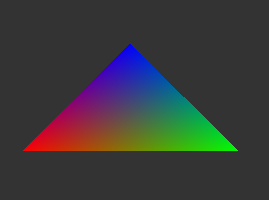
\includegraphics[width=0.4\textwidth]{Captures/Triangle.png}}
	
	\caption{Triangle d'origine}
\end{figure}
\FloatBarrier

\begin{figure}[h!]
	\adjustbox{center}{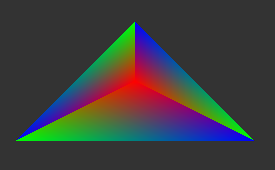
\includegraphics[width=0.4\textwidth]{Captures/InsertIn.png}}
	
	\caption{Insertion d'un point à l'intérieur d'un triangle: face split}
\end{figure}
\FloatBarrier

\begin{figure}[h!]
	\adjustbox{center}{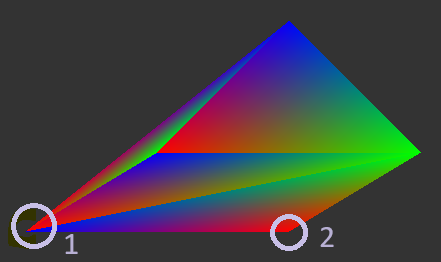
\includegraphics[width=0.4\textwidth]{Captures/InsertOut.png}}
	
	\caption{Simples insertions du point '1' puis du point '2' à l'extérieur du triangle d'origine}
	\label{InsertOut}
\end{figure}
\FloatBarrier